Il seguente codice in Python
\lstinputlisting[language=Python]{cap_1/es4/es4.m}

restituisce questo output:

\begin{tabular}{l*{6}{c}r}
i & \( x_i \) & \( y_i \)  \\
\hline
1 & 1.051709180756477  &  0.0517091807565 \\
2 & 1.005016708416795  &  0.00501670841679 \\
3 & 1.000500166708385  &  0.000500166708385 \\
4 & 1.000050001667141  &  5.0001667141e-05 \\
5 & 1.000005000006965  &  5.00000696491e-06 \\
6 & 1.000000499962184  &  4.99962183653e-07 \\
7 & 1.000000049433680  &  4.94336802603e-08 \\
8 & 0.999999993922529  &  -6.07747097092e-09 \\
9 & 1.000000082740371  &  8.27403709991e-08 \\
10 & 1.000000082740371  &  8.27403709991e-08 \\
11 & 1.000000082740371  &  8.27403709991e-08 \\
12 & 1.000088900582341  &  8.8900582341e-05 \\

\end{tabular} \\

Graficando il contenuto della tabella su di un piano XY abbiamo che \\

\textbf{ricontrollare i valore della colonna $y_i$}\\

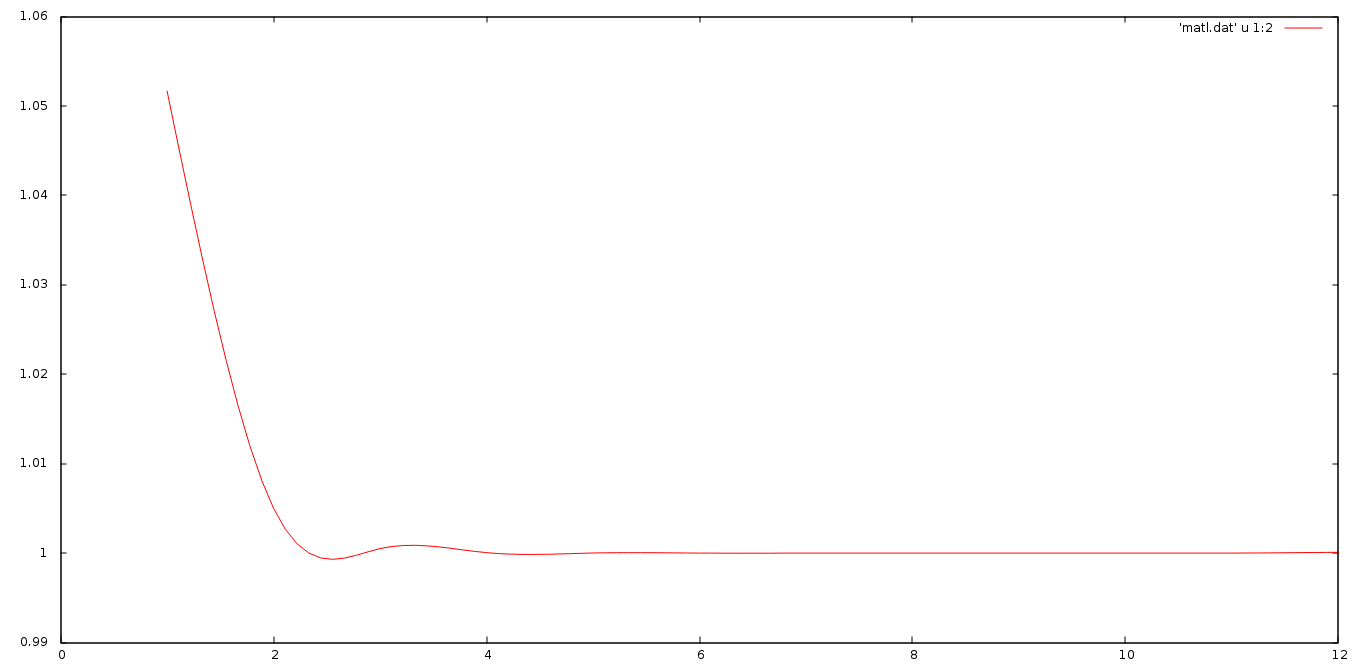
\includegraphics[scale=0.4]{cap_1/es4/matlab.png}
